\section{Knowledge-based factor}

The most commonly used knowledge-based factors are passwords and PINs.

Passwords offer several advantages: they are low-cost, easy to deploy, and have a low technical barrier for users. 
However, they also have significant drawbacks, primarily because they are susceptible to theft or snooping, guessing by unauthorized individuals, and being cracked through various methods.

To address these vulnerabilities, several countermeasures can be implemented:
\begin{itemize}
    \item \textit{Regularly changing or expiring passwords}: this reduces the risk of prolonged exposure if a password is compromised.
    \item \textit{Utilizing lengthy passwords with a diverse range of characters}: this increases complexity and makes passwords harder to crack.
    \item \textit{Ensuring passwords are not directly associated with the user}: this helps prevent predictable patterns that can be easily guessed.
\end{itemize}
Determining the most effective countermeasure requires anticipating the most probable attack in a given scenario. 
Once identified, prioritize countermeasures that users can feasibly follow and are likely to mitigate the identified threat effectively.

Countermeasures incur costs due to human limitations. 
Unlike machines, humans struggle to effectively safeguard secrets, find it challenging to remember complex passwords, and cannot adopt an unlimited number of countermeasures.
The table below summarizes the effectiveness of different countermeasures against various attack types:
\begin{table}[H]
    \centering
    \begin{tabular}{c|ccc}
                      & \textbf{Increase complexity} & \textbf{Change password} & \textbf{Not being user-related} \\ \hline
    \textit{Snooping} & $\tikzxmark$                 & $\tikzxmark$             & $\tikzxmark$          \\
    \textit{Cracking} & $\checkmark$                 & $\sim$                   & $\tikzxmark$          \\
    \textit{Guessing} & $\sim$                       & $\sim$                   & $\checkmark$    
    \end{tabular}
\end{table}

\subsection{Password complexity}
User education is critical in addressing human weaknesses, which often serve as the weakest link in security. 
This involves implementing policies to enforce strong passwords and regular password changes or expiration.
Additionally, employing password meters can help strike a balance between security and usability by guiding users in creating robust passwords.

For password complexity, it is essential to ensure that passwords contain a rich character set, including numbers, symbols, and both upper and lower-case letters. 
Moreover, passwords should be sufficiently long to resist brute-force attacks. 
Combining these elements enhances the strength of passwords and contributes to overall security.

\subsection{Password exchange}
Authentication involves sharing a secret, and several strategies can mitigate the risk of secrets being stolen: implement mutual authentication whenever feasible or utilize a challenge-response scheme, which involves exchanging random data to prevent replay attacks.
\begin{figure}[H]
    \centering
    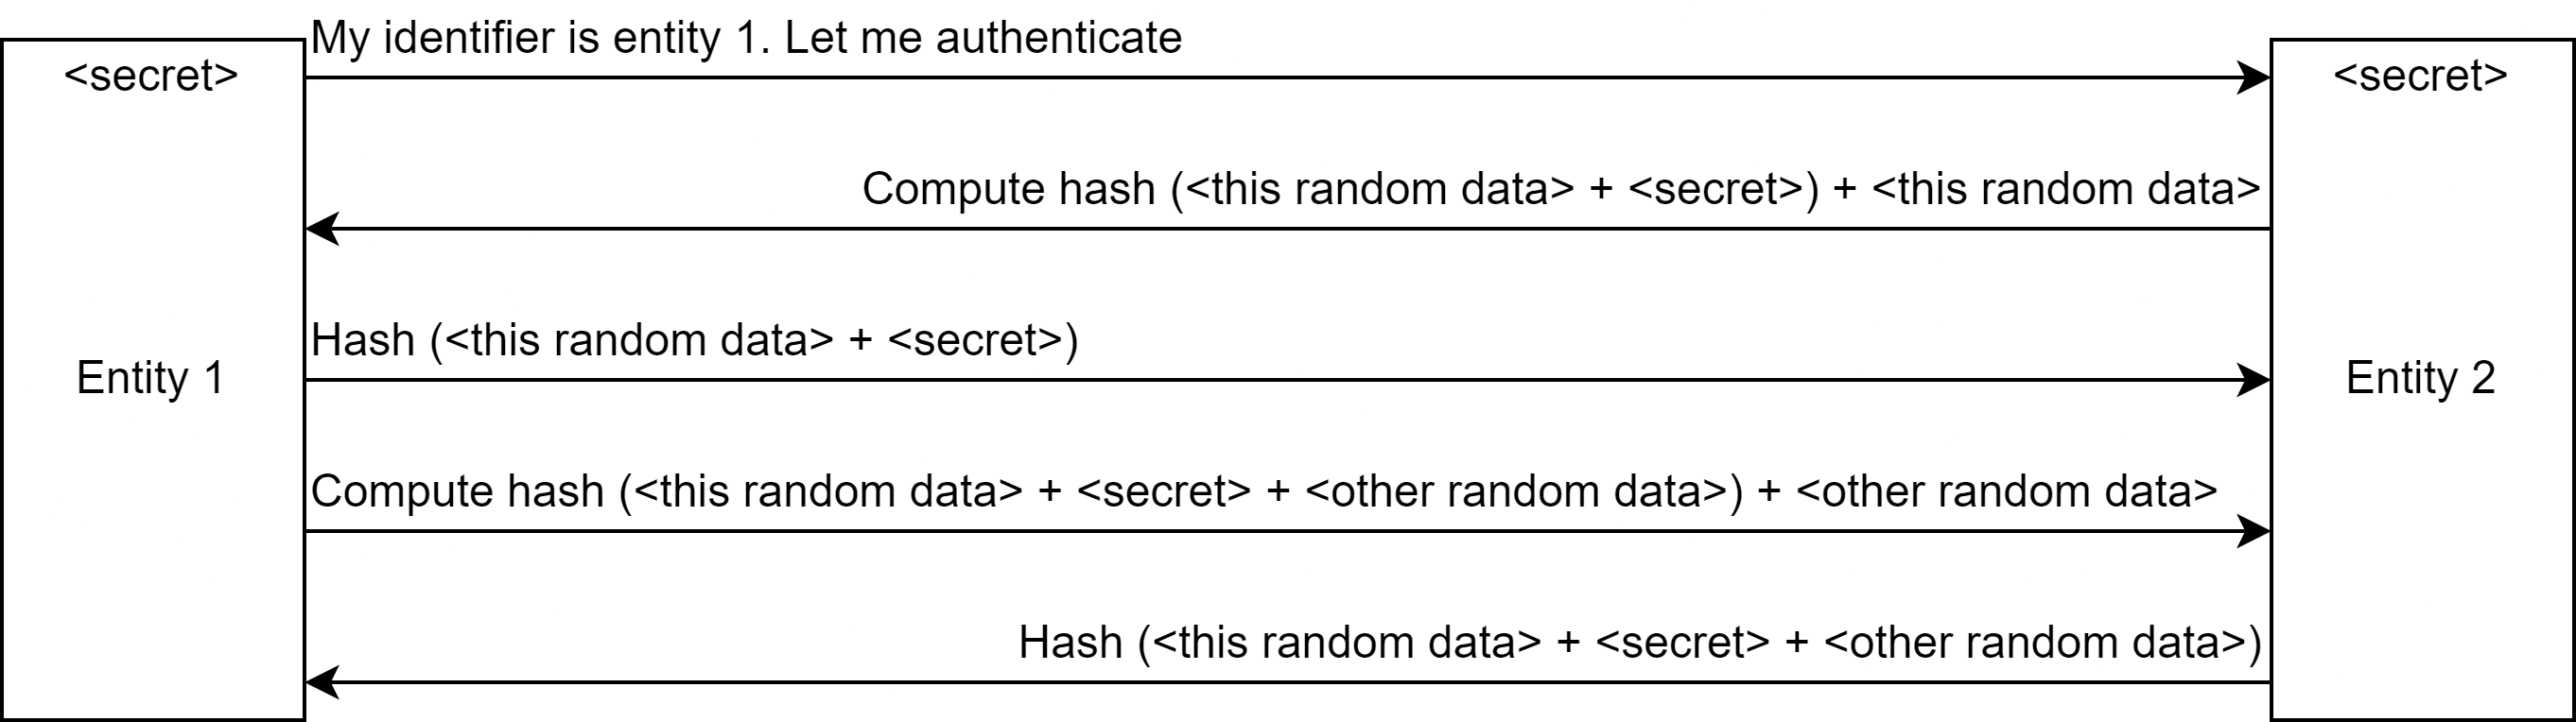
\includegraphics[width=0.75\linewidth]{images/auth2.png}
    \caption{Countermeasure costs}
\end{figure}

\subsection{Password storage}
To mitigate the risk of secrets being stolen from a file containing usernames and passwords stored by the operating system, the following measures can be implemented:
\begin{itemize}
    \item \textit{Employ cryptographic protection}: ensure that passwords are never stored in clear text. Instead, use techniques such as hashing combined with salting to mitigate dictionary attacks.
    \item \textit{Implement access control policies}: limit privileges for reading and writing to the password file to authorized users only.
    \item \textit{Avoid disclosing secrets in password-recovery schemes}: ensure that password recovery mechanisms do not inadvertently reveal sensitive information.
    \item \textit{Address caching problems}: be mindful of information stored in intermediate locations, as this can pose security risks. Regularly review and manage cached data to minimize potential exposure.
\end{itemize}
